\chapter{Marco teórico}

\section{Manipulador robótico}

\subsection{Características Scorbot ER VII}

El Scorbot-ER VII es un  manipulador robótica de cinco grados de libertad (5 DOF) diseñado para propósitos educacionales. Posee la configuración estándar de robot industrial antropomórfico (Figura \ref{cap2_scorbot}), ie. \textit{base}, \textit{shoulder} y \textit{elbow}.

\begin{figure}[ht]
  \centering
  \includegraphics[scale=0.5]{img/cap2/scorbot}
  \caption{Manipulador Scorbot ER-VII de Eshed Robotec.}
  \label{cap2_scorbot}
\end{figure}

El sistema de actuación del robot se basa en el uso de poleas reductoras seguidas de engranajes armónicos (\textit{harmonic drives}) actuados por motores de corriente continua de imanes permanentes de una corriente máxima de \SI{6,22}{\ampere} a \SI{12,0}{\volt}. La carga máxima que puede llevar el robot es de \SI{2}{\kilo\gram} (incluido el peso del efector). Esta configuración asegura que el sistema es seguro para operar fuera de una jaula de seguridad \cite{scorbot1998}.


\begin{table}[]
\centering
\begin{tabular}{|l|l|l|l|}
\hline
\multicolumn{1}{|c|}{\textbf{Eje}} & \textbf{Nombre} & \textbf{Rango} & \multicolumn{1}{c|}{\textbf{Especificaciones}} \\ \hline
\multicolumn{1}{|c|}{\multirow{5}{*}{1}} & \multirow{5}{*}{Base} & \multirow{5}{*}{310} & Voltaje: 12,0 v \\ \cline{4-4} 
\multicolumn{1}{|c|}{} &  &  & Motor Pittman-9434G697 \\ \cline{4-4} 
\multicolumn{1}{|c|}{} &  &  & Encoder HP-HEDS-5500-K11 (incremental) 96 pulsos/rev \\ \cline{4-4} 
\multicolumn{1}{|c|}{} &  &  & Reducción Harmonic gear razón 1:160 \\ \cline{4-4} 
\multicolumn{1}{|c|}{} &  &  & Transmisión Timing belt razón 1:3 \\ \hline
\multirow{5}{*}{2} & \multirow{5}{*}{Shoulder} & \multirow{5}{*}{170} & Voltaje: 12,0 v \\ \cline{4-4} 
 &  &  & Motor Pittman-9434G697 \\ \cline{4-4} 
 &  &  & Encoder HP-HEDS-5500-K11 (incremental) 96 pulsos/rev \\ \cline{4-4} 
 &  &  & Reducción Harmonic gear razón 1:160 \\ \cline{4-4} 
 &  &  & Transmisión Timing belt razón 1:3 \\ \hline
\multirow{5}{*}{3} & \multirow{5}{*}{Elbow} & \multirow{5}{*}{225} & Voltaje: 12,0 v \\ \cline{4-4} 
 &  &  & Motor Pittman-9434G697 \\ \cline{4-4} 
 &  &  & Encoder HP-HEDS-5500-K11 (incremental) 96 pulsos/rev \\ \cline{4-4} 
 &  &  & Reducción Harmonic gear razón 1:160 \\ \cline{4-4} 
 &  &  & Transmisión Timing belt razón 1:3 \\ \hline
\multirow{5}{*}{4} & \multirow{5}{*}{Wrist pitch} & \multirow{5}{*}{180} & Voltaje: 12,0 v \\ \cline{4-4} 
 &  &  & Motor Pittman-9413G698 \\ \cline{4-4} 
 &  &  & Encoder HP-HEDS-5500-K11 (incremental) 96 pulsos/rev \\ \cline{4-4} 
 &  &  & Reducción Harmonic gear razón 1:100 \\ \cline{4-4} 
 &  &  & Transmisión Timing belt razón 1:3 \\ \hline
\multirow{4}{*}{5} & \multirow{4}{*}{Wrist roll} & \multirow{4}{*}{360} & Voltaje: 12,0 v \\ \cline{4-4} 
 &  &  & Motor Pittman-9413G698 \\ \cline{4-4} 
 &  &  & Encoder HP-HEDS-5500-K11 (incremental) 96 pulsos/rev \\ \cline{4-4} 
 &  &  & Reducción Harmonic gear razón 1:100 \\ \hline
\end{tabular}
\caption{Especificaciones de articulaciones robot Scorbot ER VII.}
\label{my-label}
\end{table}


\section{Conceptos de cinemática}

Una de las tareas principales de un robot manipulador corresponde a seguir una trayectoria dejando al efector en una posición deseada. En orden de mover el robot a través de dos o más puntos de una trayectoria objetivo en un tiempo, velocidad y aceleración especificados, es necesario definir el movimiento de cada uno de los componentes del robot.

El análisis cinemático es el estudio del movimiento de los distintos elementos del robot, sin considerar las fuerzas y momentos que producen tal movimiento de los elementos.

\subsection{Cinemática directa}

Cinemática directa es el nombre que recibe el problema de encontrar la posición y orientación del efector relativo a la base del robot dados todas posiciones de las articulaciones y parámetros geométricos de los elementos que constituyen el robot. Usualmente, el sistema de referencia fijo en el efector se denomina \textit{tool frame} \cite{handbook}.

En la práctica, la cinemática directa es resuelta notando que para una cadena de elementos en serie, como es el caso del robot Scorbot, la transformada entre el sistema de referencia y el sistema fijo en el efector esta dada por la concatenación de las transformadas entre elementos adyacentes de la cadena cinemática.

\begin{equation}
T_0^5(\vec{\theta}) = T_0^1 T_1^2 T_2^3 T_3^4 T_4^5 
\end{equation}

Donde $\vec{\theta}=[\theta_1,\dotsc,\theta_5]$, $\theta_i$ corresponde al ángulo de la articulación $i$-ésima y $T_j^i$ es la transformada homogénea del elemento $i$ con respecto al sistema de referencia $j$.

\subsection{Cinemática inversa}

Por otro lado, la cinemática inversa es el nombre que recibe el problema de encontrar el valor de las posiciones de las articulaciones dada la posición y orientación del efector.
Usualmente, el cálculo de la cinemática inversa involucra la resolución de sistemas geométricos complejos que dificulta la obtención de formas cerradas, en casos donde la forma cerrada no existe se pueden emplear métodos numéricos basados en el jacobiano del sistema.

La obtención de modelos exactos de cinemática directa e inversa es tratado de forma extensa en \cite{cole2007} y \cite{predescu2015}.

\section{Controladores PID}

Aunque las nuevas y eficaces teorías y metodologías de diseño de controladores se están desarrollando continuamente en el campo del control automático, los controladores Proporcional Integral Derivativo (PID) son todavía los controladores más ampliamente utilizados en la industria debido a la ventajosa relación costo-beneficio que pueden proporcionar. De hecho, aunque son relativamente simples de usar, son capaces de lograr un desempeño satisfactorio en muchas tareas de control de procesos. De hecho, su larga historia y el \textit{know-how} que se ha desarrollado a lo largo de los años lo ha consolidado como el controlador de retroalimentación estándar \cite{practical_pid}.

Aplicar un controlador PID consiste en aplicar la suma de tres acciones de control: la acción proporcional, la acción integral y la acción derivativa. Estas acciones se describen a continuación.

\subsubsection{Control proporcional}
En control proporcional la acción de control es proporcional al error actual del sistema, como se muestra en la expresión (\ref{ctrl-kp}).

\begin{equation}\label{ctrl-kp}
u(t) = K_p e(t) = K_p(r(t)-y(t))
\end{equation}

Donde $K_p$ es la constante proporcional. El significado es directo, pues implementa la operación de incrementer la variable controlada cuando el error aumenta. La función de transferencia se muestra en la expresión (\ref{ctrls-kp}).

\begin{equation}\label{ctrls-kp}
C(s) = K_p
\end{equation}

\subsubsection{Control integral}

La acción interal es proporcional a la integral del error de control, es decir, esta dada por la expresión (\ref{ctrl-int-t}).

\begin{equation}\label{ctrl-int-t}
u(t)=K_i \int_{0}^{t}e(t)dt 
\end{equation}

Donde $K_i$ corresponde a la ganancia integral. Esta acción de control considera todos los valores pasados del error de control. La función de transferencia asociada esta dada por la ecuación ()
\begin{equation}\label{ctrl-int}
C(s)=K_i\frac{1}{s}
\end{equation}

La presencia de un polo en origen del plano complejo permite la reducción del error en estado estacionario ante una entrada o perturbación de tipo escalón. En otras palabras, la acción integral permite adaptar el valor de $u(t)$ de tal forma de alcanzar cero error en estado estacionario.

La aplicación conjunta de una acción proporcionar e integral da origen al controlador PI, ampliamente usado para resolver problemas oscilatorios de controladores On Off y error estacionario de controladores proporcionales. Si el control integral esta presente, el fenómeno de \textit{windup} puede ocurrir ante la presencia de saturación de la variable controlada.

\subsubsection{Control derivativo}

Mientras la acción de control proporcional esta basada en el valor actual del error de control y la acción integral esta basada en el los valores pasados del error de control, la acción derivativa esta basada en la predicción de los valores futuros del error de control. Una ley de control derivativa ideal se muestra en la expresión ().

\begin{equation}
u(t) = K_d \frac{de}{dt}
\end{equation}

Donde $K_d$ corresponde a la ganancia derivativa. La función de transferencia esta dada por la expresión ().
\begin{equation}
C(s) = K_d s
\end{equation}

Consideremos la expansión en serie de Taylor del error de control en $t + T_d$.

\begin{equation}
e(t + T_d) = e(t) + T_d \frac{de}{dt}
\end{equation}

Si aplicamos la ley de control proporcional a esta expresión se obtiene:

\begin{equation}
u(t) = K_p \left( e(t) + T_d \frac{de}{dt} \right)
\end{equation}

Esto corresponde naturalmente a un controlador PD. La variable controlada en $t$ esta también calculada usando una estimación del error de control en $t+T_d$. Por esta razón, se establece que el control derivativo añade elementos de control predictivo. Esto parece tener un gran potencial para mejorar el desempeño, sin embargo, existen algunos problemas en la implementación de este tipo de controladores, en especial las relacionadas con la amplificación del ruido de alta frecuencia.

\subsubsection{Discretización de controladores}

En la sección pasada se describió la función de los controladores PID continuos, gran parte de las aplicaciones de control actuales se realizan con ayuda elementos digitales, como microcontroladores o FPGA, por lo que los controladores deben ser llevados al dominio discreto para ser implementados en estas plataformas.

En términos de función de transferencia, buscamos una transformar la expresión en tiempo continuo $G(s)=\frac{B(s)}{A(s)}$ a una de tiempo discreto  $G(z)=\frac{B(z)}{A(z)}$, para lograr esto se debe encontrar la relación $s=f(z)$.

La relación $s=f(z)$ puede obtenerse considerando que para mantener estabilidad todos los polos del sistema deben ser mapeados dentro de la circunferencia unidad, de esta forma se obtiene que la relación (\ref{cap2_zmapping})\cite{oppenheim2009}.

\begin{equation}\label{cap2_zmapping}
z=e^{s T_s}
\end{equation}

Considerando una expansión de Taylor de primer orden sobre la expresión (\ref{cap2_zmapping}), se obtiene la expresión (\ref{cap2_tustin}), conocida como método de Tustin o bilineal.

\begin{eqnarray}
z &=& \frac{e^{s \frac{T_s}{2}}}{e^{-s \frac{T_s}{2}}}\\
z &\approx& \frac{1+s \frac{T_s}{2}}{1-s \frac{T_s}{2}} \label{cap2_tustin}.
\end{eqnarray}

De la expresión (\ref{cap2_tustin}) se puede obtener la relación (\ref{cap2_tustin_s}). Es común encontrar en literatura y documentación de DSP la notación $w=z^{-1}$.

\begin{eqnarray}
z &=& \frac{e^{s \frac{T_s}{2}}}{e^{-s \frac{T_s}{2}}}\\
z &\approx& \frac{1+s \frac{T_s}{2}}{1-s \frac{T_s}{2}} \label{cap2_tustin}.
\end{eqnarray}

\begin{equation}\label{cap2_tustin_s}
s \approx \frac{2}{T_s} \frac{1-z^{-1}}{1+z^{-1}} = \frac{2}{T_s} \frac{1-w}{1+w}
\end{equation}

\subsubsection{Implementación de controladores digitales}

Para describir la implementación de un controlador digital, consideremos un control integral, donde $k_i$ corresponde a la contante integral:

\begin{eqnarray}
C(s) &=& k_i \frac{1}{s}\\
C(s)_{s=\frac{2}{T_s} \frac{1-w}{1+w}} &=& \frac{k_i T_s}{2} \frac{1+w}{1-w} \\
C(w) &=& \frac{  \frac{k_i T_s}{2} w +  \frac{k_i T_s}{2} }{(-1)w+1} 
\end{eqnarray}

Considerando que un esquema de control realimentado, se tiene que $C(w) = \frac{u(w)}{e(w)}$, donde $u(w)$ corresponde a la salida del controlador y $e(w)$ al error, ambos en dominio discreto.

\begin{eqnarray}
\frac{u(w)}{e(w)} &=& \frac{  \frac{k_i T_s}{2} w +  \frac{k_i T_s}{2} }{(-1)w+1} \\
u(w)-u(w)w &=& e(w) \frac{k_i T_s}{2} w +  e(w) \frac{k_i T_s}{2} \label{cap2_eq_diff_w}
\end{eqnarray}

Aplicando transformada $Z$ inversa sobre la expresión (\ref{cap2_eq_diff_w}) se obtiene la ecuacion de diferencia:

\begin{eqnarray}
u(n)- u(n-1) &=&  \frac{k_i T_s}{2}(e(n)+e(n-1)) \\
\Delta u(n) &=& k_i \left( T_s \, \frac{e(n)+e(n-1)}{2} \right) \label{cap2_eq_control_int}
\end{eqnarray}

De la expresión \ref{cap2_eq_control_int}, muestra que el cambio en la salida del controlador esta dado por la integral del error. Notamos que podemos reescribir la ecuación de diferencia de la siguiente forma:

\begin{eqnarray}
u(n) &=&  \frac{k_i T_s}{2} e(n) + \alpha(n-1) \\
\alpha(n) &=& u(n) + \frac{k_i T_s}{2} e(n)
\end{eqnarray}

Esta representación nos indica que para implementar el controlador deseado solo se necesita almacenar un estado $\alpha(n)$, pues el corresponde a sistema de primer orden. La implementación en diagrama de bloques se muestra en la Figura \ref{cap2_block_integral}.

\begin{figure}[H]
  \centering
  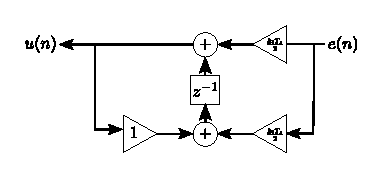
\includegraphics[scale=1.5]{img/cap2/block_pi}
  \caption{Diagrama de bloques controlador integral.}
  \label{cap2_block_integral}
\end{figure}

Esta represetación se denomina forma Directa II versión transpuesta, la cual es óptima con respecto a los elementos de retardo necesarios para la implementación, pues los polos y ceros comparten los elementos de retardo, lo que finalmente se traduce en el uso de una estructua de datos más compacta en el microcotrolador. De forma más general, la función de transferencia $H(w)$ de un filtro digital puede expresarse como muestra la expresión (\ref{cap2_filtro_digital}) y representarse en diagrama de bloques según la Figura (\ref{cap2_td2}).

\begin{equation}
H(w) = \frac{\sum_{k=0}^{M} b_k \, w^k}{1-\sum_{k=1}^{N} a_k \, w^k}\label{cap2_filtro_digital}
\end{equation}

\begin{figure}[H]
  \centering
  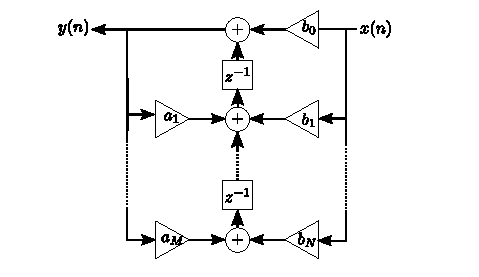
\includegraphics[scale=1.2]{img/cap2/tdf2}
  \caption{Diagrama de bloques para representación Directa II versión transpuesta.}
  \label{cap2_td2}
\end{figure}

\section{Motores de corriente continua}

El motor de corriente continua (CC) es la máquina eléctrica empleada en aplicaciones de potencia y tracción. Su sencillo accionamiento y estructura de control han permitido que siga vigente hasta nuestros días, a pesar de ser constructivamente más complejo que los que motores BLDC y requerir mantenimiento. Su velocidad fácilmente controlable y posibilidad de girar en ambos sentidos, lo  que permite aplicaciones de servo accionamientos y tracción.

El funcionamiento del motor de CC se basa en la fuerza generada por la interacción de un campo magnético inmóvil y uno generado por una bobina móvil (armadura), montada sobre un eje de rotación. La bobina móvil es alimentada a través de un sistema de escobillas y delgas para invertir la dirección de la corriente y, por consiguiente, el sentido del campo magnético generado, logrando que el torque resultante sea siempre favorable al sentido de giro \cite{vargas2006}. En la Figura \ref{cap2_motorcc} se muestra la bobina dentro de un campo magnético fijo de dirección horizontal.

\begin{figure}[H]
    \centering
    \begin{subfigure}[b]{0.48\textwidth}
            \includegraphics[width=\textwidth]{img/cap2/motor_cc1.png}
            \caption{Bobina elemental del motor de CC dispuesta sobre un eje de giro y alimentada a través de las escobillas.}
    \end{subfigure}
    ~
    \begin{subfigure}[b]{0.48\textwidth}
            \includegraphics[width=\textwidth]{img/cap2/motor_cc2.png}
            \caption{Bobina montada en un rotor dentro de un campo magnético fijo cuya dirección es perpendicular al eje de giro.}
    \end{subfigure}
    \caption{Bobinas del motor de CC}
    \label{cap2_motorcc}
\end{figure}


El flujo de campo $\phi_f$ de dirección fija generado por el estator puede ser producido por un devanado o imanes permanentes, como es el caso del los motores que posee el manipulador Scorbot ER-VII. El uso de imanes permanentes establece un flujo de campo $\phi_f$ constate, esto mejora la eficiencia de la máquina, pero limita la velocidad de operación de la misma, pues no es posible operar a flujo debilitado.

En un motor de CC, el par de torsión electromagnético $T_m$ es producto de la interacción entre el flujo de campo $\phi_f$ y la corriente de armadura $i_a$.

\begin{eqnarray}
T_m &=& k_f \phi_f i_a \\
T_m &=& k_T i_a
\end{eqnarray}

Donde $k_f$ es la constante de par de torsión del motor. Como $\phi_f$ es constante, se usa $k_T= k_f \phi_f$.

En el circuito del inducido se produce una fuerza contraelectromotriz por la rotación de conductores de inducido a una velocidad $\omega_m$ en la presencia de un flujo de campo $\phi_f$.

\begin{equation}
e_a = k_e \phi_f \omega_m
\end{equation}

Donde $k_e$ es la constante de voltaje del motor. Se puede demostrar \cite{mohan}, que usando unidades SI $k_e \phi_f = k_T$, de esta forma fuerza contraelectromotriz, también denominada reacción de armadura, esta dada por la Ecuación \ref{eq_reaccion_armadura}.

\begin{equation}\label{eq_reaccion_armadura}
e_a = k_T \omega_m
\end{equation}

En la práctica se aplica una fuente de voltaje controlable $v_t$ a los terminales de inducido para establecer una corriente de armadura $i_a$. Por tanto, la corriente $i_a$ en el circuito de inducido se determina por $v_t$, la fuerza contraelectromotriz $e_a$, la resistencia del devanado del inducido $R_a$ y la inductancia del devanado del inducido $L_a$ se ralacionan como muestra la Ecuación \ref{eq_armadura}, esta ecuación se ilustra como circuito equivalente en la Figura \ref{cap2_dc_motor}.

\begin{equation}\label{eq_armadura}
v_t = e_a + R_a i_a + L_a \dv{i_a}{t}
\end{equation}

La ecuación anterior determina el comportamiento eléctrico del motor de corriente continua, el comportamiento mecánico esta dado por la Ecuación \ref{eq_mecanica}, donde se ve la interacción del motor con la carga mecánica.

\begin{equation}\label{eq_mecanica}
T_m = T_l + B \omega_m + J \dv{\omega_m}{t}
\end{equation}

Donde $J$ y $B$ son la inercia y amortiguamiento equivalente total, respectivamente, de la combinación motor carga y $T_l$ es el par de torsión de trabajo equivalente de la carga.

\begin{figure}[H]
  \centering
  \includegraphics[scale=0.3]{img/cap2/dc_motor_circuit}
  \caption{Circuito equivalente de un motor de corriente continua.}
  \label{cap2_dc_motor}
\end{figure}

Un hecho importante de la actuación robot manipuladores corresponde a la naturaleza dinámica de la carga mecánica de cada articulación actuada, esto debido efectos gravitatorios y dinámicos generados por otros enlaces en movimiento de la cadena cinemática.


\subsection{Control de motores de corriente continua}

Como se mostró anteriormente, el torque producido por el motor de CC es proporcional a la corriente de armadura, dado que el objetivo es el control de las variables mecánicas (\textit{i.e.} torque, velocidad) es directo establecer como primera estructura el control la corriente de armadura. Para el control de la corriente de armadura es necesario que $v_t$ esté conectado a una fuente de voltaje controlable, esto se logra utilizando un circuito llamado convertidor de puente completo o puente H, el cual utiliza una estructura de puente que permite la conducción en ambos sentidos, tal como se muestra en la Figura \ref{cap2_punteh}.

\begin{figure}[ht]
  \centering
  \includegraphics[scale=.2]{img/cap2/puenteh}
  \caption{Configuración del puente H.}
  \label{cap2_punteh}
\end{figure}

El uso de modulación PWM en el encendido de los transistores permite controlar el valor efectivo de la tensión de alimentación del motor CC. El diseño de estos dispositivos de potencia es un trabajo complejo, pues requiere la correcta elección de semiconductores, un \textit{layout} capaz de soportar altas corrientes y evitar la aparición de inductancias parásitas.

Dada la naturaleza inductiva del circuito de armadura, la modulación PWM de la tensión no establece un régimen de corriente pulsante, si no cierto nivel de rizo en la corriente estableciendo un estado que se denomina de corriente plana. Si el motor posee una baja inductancia de armadura, es posible que salga del régimen de corriente plana y se produzcan torques pulsantes. Este efecto puede ser reducido aumentando la frecuencia de conmutación o la conexión de inductancias en serie.

Afortunadamente, dado la gran demanda de estos dispositivos por parte de la industria automovilística, fabricantes de semiconductores entregan soluciones acorde a los requerimientos.

\section{Interfaces hápticas}

Los dispositivos hápticos son capaces de proporcionar una retroalimentación de fuerza al usuario que lo emplea, de esta forma complementan sistemas de operación visuales al entregar más información al operador. Esta tecnología puede aplicarse a múltiples sectores con el fin de facilitar su ejecución: medicina, realidad virtual, modelado, robótica, entre otras.

\subsection{Phantom Omni \texttrademark}

Phantom Omni \texttrademark (actualmente Geomatic\textregistered \, Touch \texttrademark) es un dispositivo háptico de seis grados de libertad (6 \textit{DOF}) desarrollado por Sensable\textregistered, permite leer la posición de sus seis articulaciones y posee tres actuadores conectados a los tras primeras articulaciones, permitiendo la aplicación de fuerzas, que solo pueden controlar la posición del \textit{stylus} en el espacio cartesiano.

\begin{figure}[ht]
  \centering
  \includegraphics[scale=.2]{img/cap2/phantom_omni}
  \caption{Phantom Omni \texttrademark.}
  \label{cap2_phantom}
\end{figure}

Un aspecto importante del diseño es el desacople entre la posición y orientación \cite{beckman2007}, las tres primeras articulaciones son usadas para posicionar el \textit{stylus} y las restantes establecen la orientación del mismo. Los ejes de giro de estas últimas tres articulaciones se intersectan en un mismo punto, por lo que se puede interpretar como una articulación esférica.

La configuración cinemática del Phantom Omni \texttrademark \, es similar a la del robot Scorbot ER VII, pues poseen una cadena cinemática con una base, dos elementos articulados que se mueven en un plano y una muñeca. La mayor diferencia entre ellos, aparte de su tamaño, radica en que el dispositivo háptico posee 6 grados de libertad y solo tres articulaciones son actuadas, por otro lado el robot posee solo 5 grados de libertad, todos ellos actuados. 

\section{Bus de campo}

Los primeros enlaces de datos estaban limitados a la conexión entre dos dispositivos, esto se traducía en que cada nuevo dispositivo debía ser conectado directamente al controlador en una topología de estrella. Esto llevó al desarrollo de buses de campo (\textit{fieldbuses}), definidos en el estándar IEC 61158, permitiendo la conexión múltiples nodos usando el mismo cable, lo que se denomina \textit{multidrop bus}. Esto trajo consigo cableados más simples y redes más modulares. Compartir un bus entre varios nodos requiere de un protocolo que maneje de forma adecuada el envío y recepción de datos de los dispositivos conectado al bus.

Un esquema de control distribuido requiere de un bus de campo capaz de compartir información con los dispositivos de forma determinista, pues los algoritmos de control e información critica deben cumplir estrictos requerimientos temporales (\textit{timming}). Algunos requerimientos clásicos se describen a continuación:

\begin{itemize}

\item Frecuencia de actualización: Controladores obtienen información de sensores y envían comandos a los actuadores de manera periódica, usualmente, a una frecuencia fija. Esta frecuencia depende de la aplicación en particular, por ejemplo es usual que lazos de control de servomotores tengan frecuencias de actualización cercanas a \SI{1}{kHz}.

\item \textit{Jitter}: Corresponde a la variabilidad temporal durante el envío de señales digitales. La presencia de \textit{jitter} en el bus de campo puede tener efectos no deseados, siguiendo el ejemplo anterior, un \textit{jitter} de \SI{1}{\milli\second} puede considerarse inaceptable, pues es del orden del tiempo de actualización.

\end{itemize}


\subsection{EtherCAT}

EtherCAT (\textit{Ethernet for Control Automation Technology}) es un bus de campo de código abierto, fue creado con el fin de emplear el potencial Ethernet y mejorar las áreas donde este falla al momento de implementarse en redes de control, de esta forma introduce comportamiento determinista y reducción en el tiempo de procesamiento de paquetes de datos pequeños.

\subsubsection{Estructura maestro-esclavo}

EtherCAT emplea una estructura maestro-esclavo donde cada dispositivo es conectado en cadena uno tras otro como se muestra en la Figura \ref{cap2_ethercat_chain}.

La transmisión es iniciada por el dispositivo maestro, el mensaje es transmitido a la cadena de esclavos donde cada dispositivo puede leer o escribir en el mensaje antes de pasarlo al siguiente dispositivo. Una vez el mensaje alcanza el último dispositivo esclavo, éste lo envía hacia el maestro a través de la cadena. Desde fuera, de la estructura formada por la cadena de esclavos se puede considerar como un nodo Ethernet.

\begin{figure}[ht]
  \centering
  \includegraphics[scale=.5]{img/cap2/ethercat_chain}
  \caption{Estructura maestro esclavo de EtherCAT.}
  \label{cap2_ethercat_chain}
\end{figure}

\subsubsection{Enlace de datos}

Dado que cada dispositivo esclavo debe leer el mensaje antes de saber que hacer con él, este proceso puede introducir una cantidad de calculo que debe realizar el software y que va en desmedro del rendimiento aplicación principal. Para evitar eso cada esclavo esta equipado con \textit{EtherCAT Slave Controller} (ESC), el cual procesa el mensaje recibido en hardware, reduciendo de forma significativa el tiempo de procesamiento en el esclavo. Gracias a esto, el dispositivo esclavo empieza la transmisión al siguiente nodo cuando aún esta recibiendo el mensaje. El ESC contiene toda la funcionalidad de la capa de enlace de datos especificada por el estándar, la capa de aplicación depende del tipo de ESC usada.

Dado el enlace de datos se realiza por hardware, los dispositivos esclavos deben contar con hardware especializado para usar el bus de campo EtherCAT. Usualmente existen dos alternativas para la integración de EtherCAT en un dispositivo: uso de un EtherCAT ASIC o integración de un IP usando una FPGA. Actualmente, esta tecnología se integra en microcontroladores, permitiendo diseños más compactos y económicos (Figura \ref{cap2_ethercat}).

\begin{figure}[H]
  \centering
  \begin{subfigure}[b]{0.4\textwidth}
    \includegraphics[width=0.6\textwidth]{img/cap2/ethercat_asic.png}
    \caption{EtherCAT ASIC de Beckhoff Automation GmbH.}
    \end{subfigure}%
    ~
  \begin{subfigure}[b]{0.4\textwidth}
    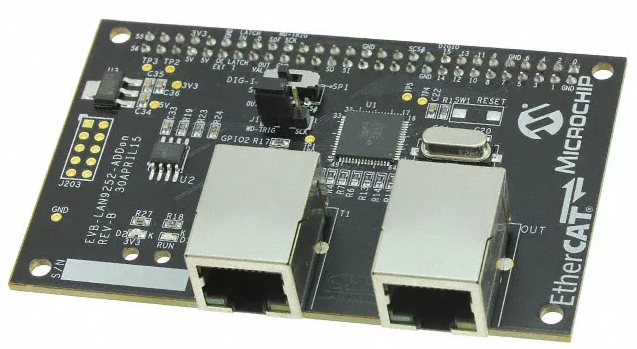
\includegraphics[width=\textwidth]{img/cap2/microchip_lan9252}
    \caption{Placa de desarrollo del microcontrolador LAN9252 de Microchip puerto EtherCAT integrado}
    \end{subfigure}
  \caption{Alternativas de integración de EtherCAT en dispositivos.}
  \label{cap2_ethercat}
\end{figure}

\section{Componentes de software}

\subsection{ROS}

Robot Operating System (ROS) \cite{quigley2009} es un  framework para el desarrollo de aplicaciones robóticas, ofrece herramientas, librerías, abstracción de hardware, controladores de dispositivos, visualizadores, comunicación entre procesos, gestión de paquetes, entre otros.

A pesar de su nombre, ROS no es un sistema operativo propiamente dicho, es más bien un middlewere que se integra en sistemas GNU/Linux como Ubuntu. Una de sus principales ventajas es su amplia comunidad y que se encuentra bajo la licencia BSD, que permite el uso del software en aplicaciones comerciales. Fue desarrollado en 2007 por el Laboratorio de Inteligencia Artificial de Stanford bajo el nombre de \textit{switchyard}, luego su desarrollo continuó en el laboratorio de investigación robótico Willow Garage, actualmente la OSRF (\textit{Open Source Robotics Foundation}) es la encargada de mantener las herramientas básicas de ROS.

Uno es los aspectos más importantes de ROS es interfaz para la comunicación entre procesos. Un nodo, unidad de software básica en ROS, puede publicar o suscribirse a un tópico. En este tópico se escriben/leen mensajes que han sido depositados por otros nodos. Puede haber varios publicadores y subscriptores sobre el mismo tópico concurrentemente. Un único nodo puede publicar y subscribiese a múltiples tópicos.

Los mensajes son estructuras de datos que soportan tipos primitivos como
enteros, punto flotante, arreglos de primitivas y constantes. Adicionalmente los mensajes pueden estar compuestos por otros mensajes y por arreglos de mensajes, dando la profundidad que se requiera.

Otro elemento primordial lo constituyen los servicios, estos se definen mediante un par de mensajes, unos para la solicitud (\textit{request}) y otro para la respuesta (\textit{response}). Un nodo ofrece un servicio bajo un nombre y un cliente llama al servicio enviando un mensaje de solicitud y esperando a la respuesta.

\section{Evaluación del sistema}

Para la evaluación del sistema se propone el uso de una aplicación de teleoperación háptica donde operador podrá:

\begin{itemize}

\item Mover de forma continua el robot manipulador usando la interfaz hápica Phantom Omni \texttrademark.
\item Obtener \textit{feedback} hápico considerando variables internas del robot, como la posición actual.
\item Interactuar de forma hápitica con objetos, previamente definidos, en el espacio de trabajo del robot.

\end{itemize}
